\chapter{系统设计}\label{chap:design}

\section{系统总体架构设计}

本系统采用典型的分层架构设计模式，自上而下划分为表现层、接口层、业务逻辑层以及数据存储层。各层职责明确，形成高内聚、低耦合的系统结构，便于开发维护与功能扩展。系统总体架构如\figref{fig:system-architecture}所示。

\begin{figure}[!htbp]
  \centering
  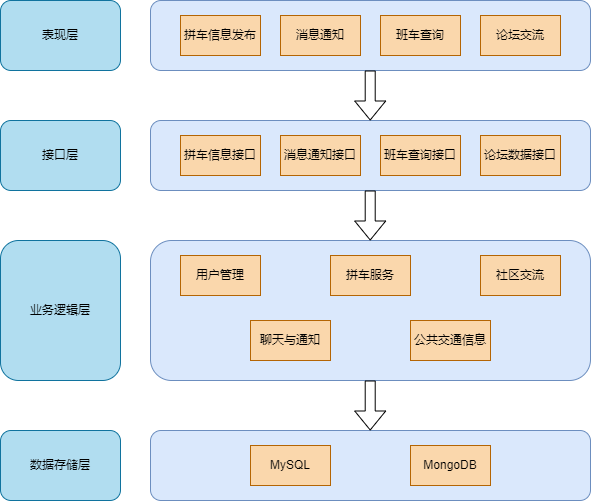
\includegraphics[width=0.94\textwidth]{figures/fig-4-1-system-architecture.png}
  \caption{系统总体架构图}
  \label{fig:system-architecture}
\end{figure}

表现层由微信小程序构成，是用户直接交互的界面层。该层承担所有校园出行相关信息的呈现、操作输入及交互响应，包括班车信息查询、拼车信息发布与匹配、社区交流及即时消息功能。表现层通过界面组件和数据绑定将系统提供的功能直观呈现给用户，同时负责初步数据验证，如表单输入检查、日期和时间范围校验等，以减轻后端负担。

通过良好的界面设计与用户体验优化，表现层实现了信息展示的直观性和操作的便捷性，使用户能够快速获取所需的出行服务。

接口层位于表现层与业务逻辑层之间，是前后端通信的桥梁。该层通过统一的RESTful API规范，将前端的请求准确路由至对应的业务模块，同时负责用户身份认证、权限校验和请求参数的初步处理，确保每一次操作均在合法范围内执行。接口层通过标准化的数据交换格式返回处理结果，既保证了前端调用的简便性，也为后端服务的独立部署和模块扩展提供了支持。

接口层还承担日志记录与异常捕获功能，对请求流程进行监控，为系统维护和故障排查提供依据。

业务逻辑层是系统的核心部分，由Spring Boot微服务组成，包括用户管理、拼车服务、社区交流、公共交通信息以及聊天与通知五大功能模块。用户管理模块负责用户注册、登录、信息维护以及信用分管理，保障身份认证的安全性和用户数据的一致性；拼车服务模块是系统的核心，通过二层匹配算法和基于随机森林的推荐机制，对用户发布的拼车信息进行智能筛选和排序，提升拼车成功率，同时实现行程全生命周期管理，包括发布、申请、审批、行程完成及反馈统计；社区交流模块实现帖子管理、评论互动和搜索功能，为校园用户提供信息交流和经验分享平台；公共交通信息模块集中管理校内班车及北安跨线公交数据，为用户提供准确、及时的出行参考；聊天与通知模块则提供即时消息服务和会话管理功能，保证用户间的高效沟通。业务逻辑层在处理业务流程时，严格遵循系统规则，实现数据校验、事务管理和算法计算，为前端提供可靠的操作接口。

数据存储层负责系统的数据持久化管理，采用MySQL和MongoDB混合方案。MySQL用于存储结构化数据，如用户信息、拼车订单和行程反馈等，以确保事务的一致性和完整性；MongoDB用于管理非结构化数据，如社区帖子、评论以及聊天消息，适应数据格式多样性和高并发访问需求。数据存储层的设计充分考虑校园出行场景下的数据需求，通过这种混合方案保证系统稳定运行。

通过上述分层设计，系统在保证功能完整性的同时实现了清晰的层次结构和模块职责划分。表现层专注用户体验，接口层保障数据交互安全可靠，业务逻辑层处理复杂的业务流程与算法计算，数据存储层提供高效稳定的数据管理支持。各层协同工作，使校内综合交通平台在高并发访问环境下仍能保持良好的性能与扩展性，为系统的持续优化和功能扩展提供了坚实基础。

\section{系统模块设计}

系统模块设计以校园综合交通场景为核心，采用微服务架构将各项功能进行独立封装与逻辑划分。模块之间通过RESTful接口进行数据交互，各模块职责明确、内聚性高，同时保证系统可扩展性和维护性。本系统主要划分为用户管理、拼车服务、社区交流、聊天与通知以及公共交通信息五大模块。

\subsection{用户管理模块}

用户管理模块是系统的基础模块，主要负责用户身份认证、个人信息维护以及信用统计管理。用户管理模块内部主要由控制层、业务层、数据访问层及工具类协同完成，其核心类关系如\figref{fig:user-class-diagram}所示。

\begin{figure}[!htbp]
  \centering
  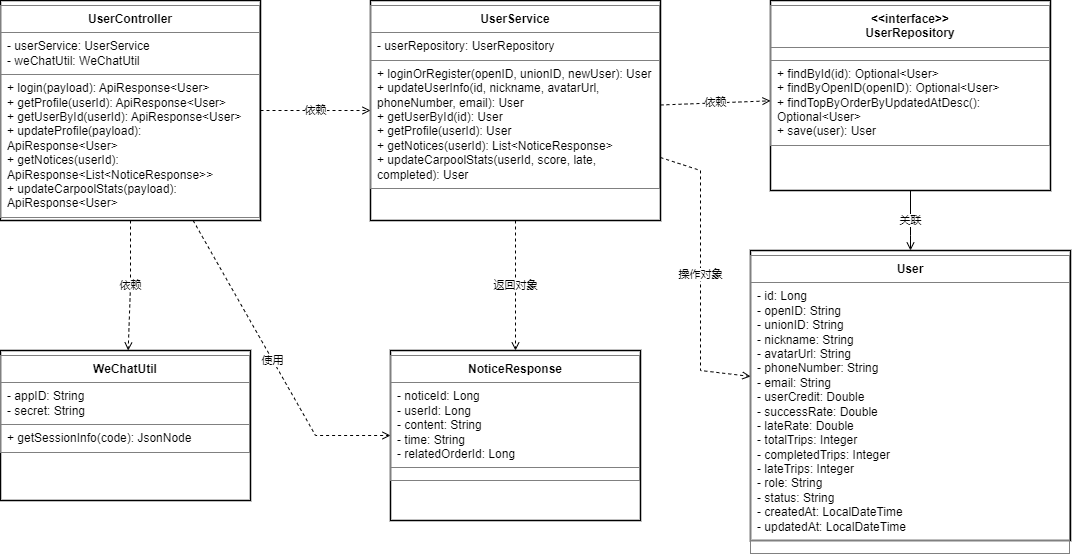
\includegraphics[width=0.96\textwidth]{figures/fig-4-2-user-class-diagram.png}
  \caption{用户管理模块类图}
  \label{fig:user-class-diagram}
\end{figure}

在校园出行场景中，用户是所有业务流程的核心，系统通过微信授权实现登录验证，确保用户身份的安全可靠。同时，该模块提供个人资料管理功能，包括昵称、头像、联系方式等信息更新和查询，使用户能够维护完整的个人档案。

为了支持拼车业务的信用体系，用户管理模块记录用户参与拼车的总次数、完成率及迟到率等指标，并在行程完成后根据反馈数据更新信用分和相关统计信息。模块设计强调数据的完整性和一致性，通过逻辑约束和接口调用保证用户信息在系统中各模块间的可访问性和实时性。

\subsection{拼车服务模块}

拼车服务模块是系统核心功能模块，负责实现拼车信息的发布、查询、匹配、申请管理以及行程反馈。模块内部设计围绕拼车完整生命周期展开，从用户发布拼车需求开始，到其他用户提交加入申请，车主审批，再到行程完成及反馈统计，形成闭环业务流程。

为提高拼车匹配效率，模块引入二层匹配机制和基于随机森林算法的推荐策略，通过分析用户历史出行记录、信用分、路线匹配度及时间偏好，实现智能排序与个性化推荐。在行程完成后，模块提供评价接口用于更新用户信用及成功率统计，从而形成动态调整的信用体系。模块内部逻辑严格控制订单状态、座位数量及申请审批流程，确保业务操作的准确性和一致性。

拼车服务模块涉及订单、申请、反馈及外部协同组件等多个对象，其核心类关系如\figref{fig:carpool-class-diagram}所示。

\begin{figure}[!htbp]
  \centering
  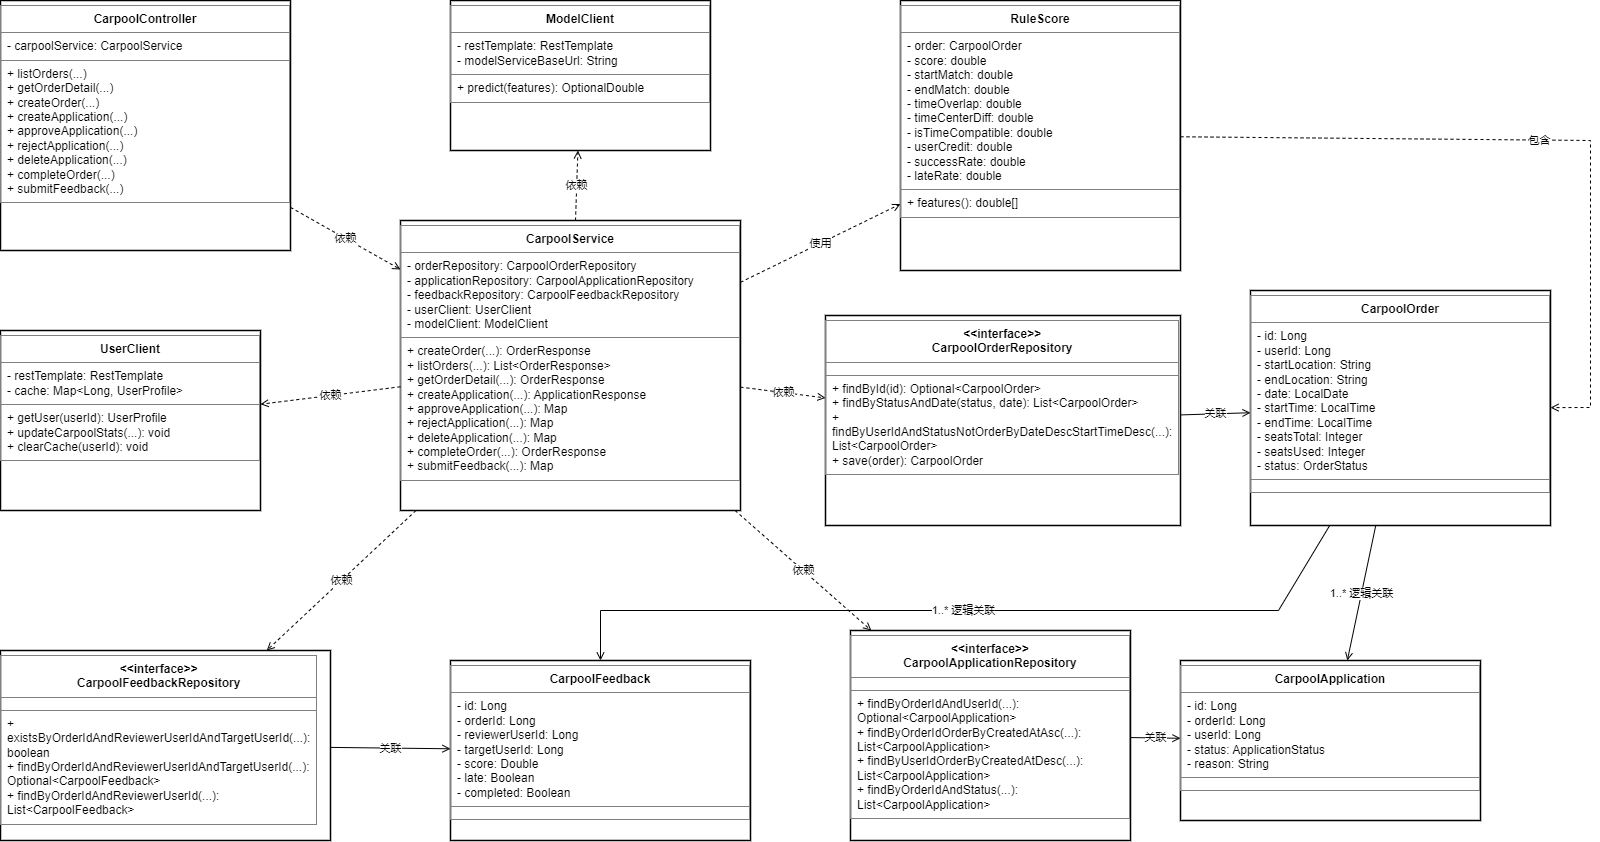
\includegraphics[width=0.96\textwidth]{figures/fig-4-3-carpool-class-diagram.png}
  \caption{拼车服务模块类图}
  \label{fig:carpool-class-diagram}
\end{figure}

从\figref{fig:carpool-class-diagram}可以看出，拼车服务模块以订单实体为中心，通过申请实体和反馈实体扩展完整业务流程，并通过用户服务调用组件和模型服务调用组件实现跨服务协同。在业务交互层面，用户申请加入拼车订单时的核心对象调用顺序如\figref{fig:application-sequence}所示。

\begin{figure}[!htbp]
  \centering
  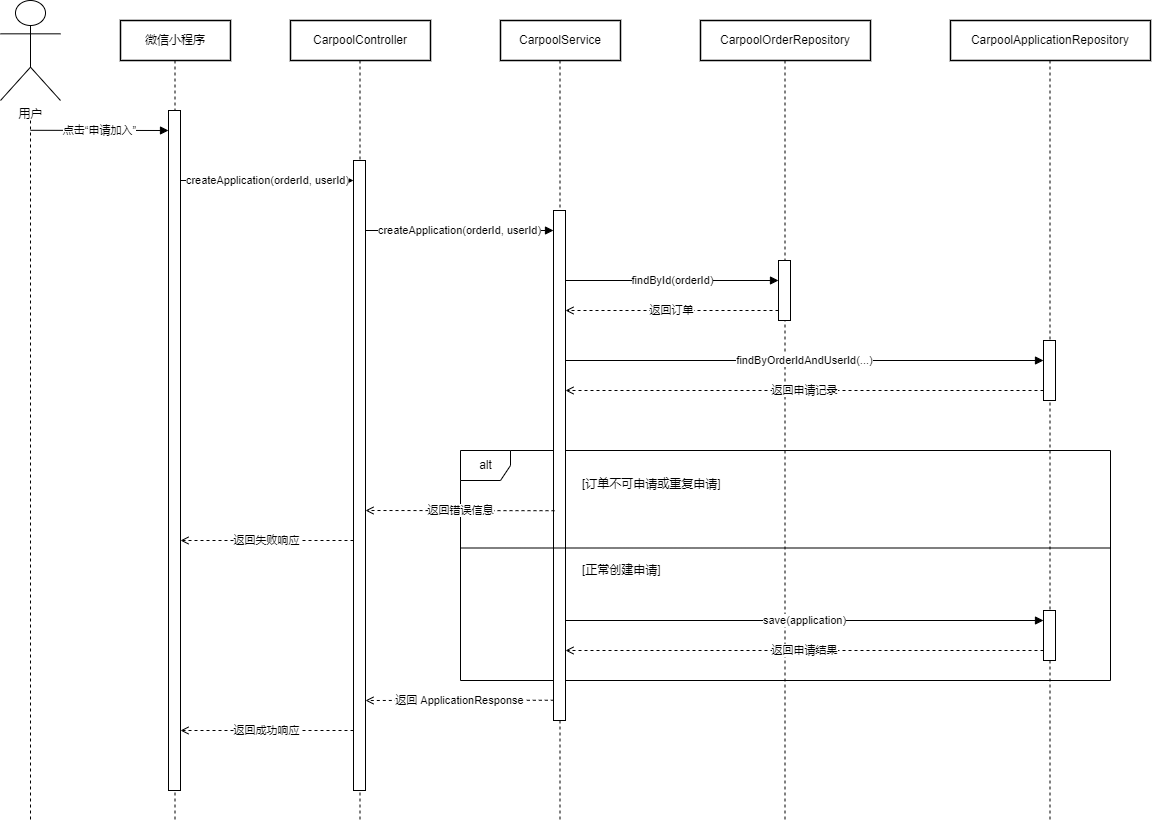
\includegraphics[width=0.94\textwidth]{figures/fig-4-4-application-sequence.png}
  \caption{拼车申请处理时序图}
  \label{fig:application-sequence}
\end{figure}

该时序图体现了拼车申请在控制层、业务层和数据访问层之间的调用顺序，也说明了系统在申请校验、重复判断和数据保存方面的处理逻辑。拼车匹配查询是系统核心业务之一，其在规则筛选与模型排序阶段的对象交互过程如\figref{fig:matching-sequence}所示。

\begin{figure}[!htbp]
  \centering
  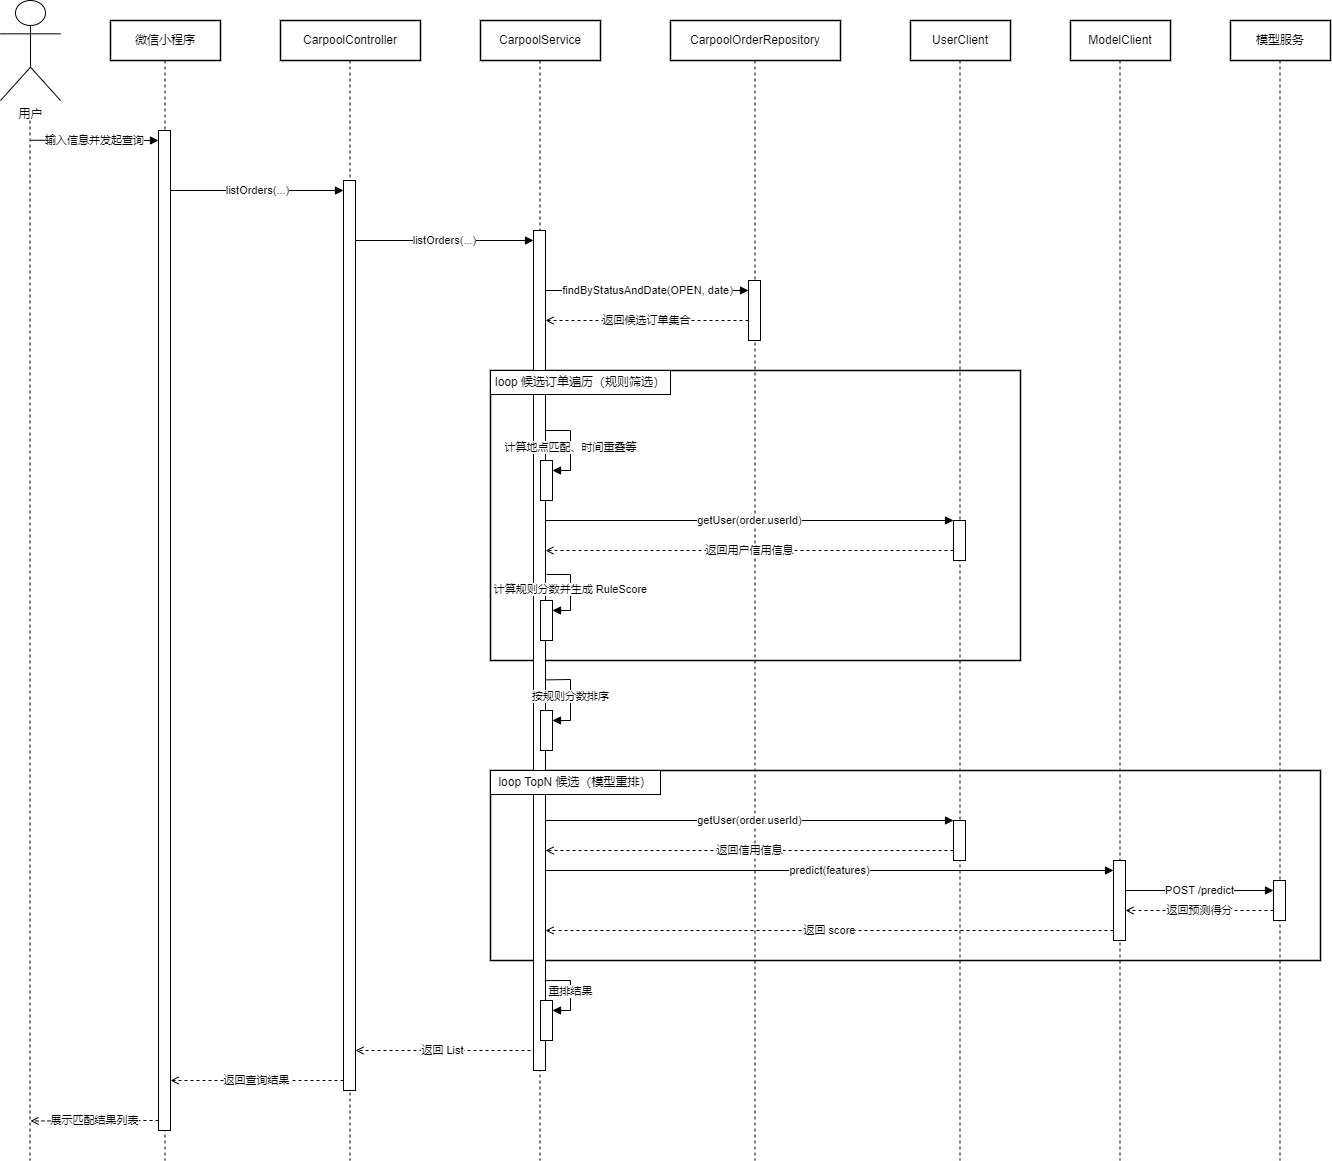
\includegraphics[width=0.94\textwidth]{figures/fig-4-5-matching-sequence.png}
  \caption{拼车匹配查询时序图}
  \label{fig:matching-sequence}
\end{figure}

由\figref{fig:matching-sequence}可见，系统在接收查询请求后，先完成候选订单筛选和特征计算，再对高质量结果调用模型服务进行排序，从而体现出拼车匹配业务的二层处理机制。

\subsection{社区交流模块}

社区交流模块为校园用户提供信息交流和经验分享的平台。模块主要支持帖子发布、评论互动及点赞功能，同时允许上传多媒体附件以增强信息表达能力。模块设计充分考虑校园社交需求，通过高效的内容存储与检索机制，实现帖子及评论的快速展示和分页加载。

模块内部通过逻辑约束保证用户对内容的操作权限，例如用户只能删除自己发布的帖子或评论，点赞操作可切换状态而不产生重复记录。模块还设计了统计字段用于快速显示点赞数和评论数量，提高列表页面的响应效率。整个模块的设计旨在增强用户互动体验，同时保持数据结构的灵活性和可扩展性。

\subsection{聊天与通知模块}

聊天与通知模块提供用户之间的即时通信功能，系统以单聊功能为主，并预留群聊扩展接口。模块实现了会话管理、消息发送与接收、已读标记及删除操作，同时为群聊提供成员管理功能。

模块内部采用嵌套文档结构存储会话成员信息和消息状态，使每条消息可以维护不同用户的已读和删除状态。在校园出行场景中，该模块确保乘客与车主之间、用户之间的即时沟通，支持跨模块通知，如拼车申请结果和行程反馈提示。模块设计注重实时性与数据一致性，通过业务逻辑控制保证消息状态的准确性和可靠性。

\subsection{公共交通信息模块}

公共交通信息模块提供校内班车及北安跨线公交信息查询服务，为用户出行提供基础数据支持。模块存储和管理完整的班车线路、时刻表及区段信息，并提供接口以查询最近发车时间或整条线路的完整时刻表。通过结构化数据存储和标准化接口，公共交通信息模块为用户提供准确、及时的出行参考，同时为拼车服务模块提供基础数据支持，增强系统整体的可用性和用户体验。

\section{数据库设计}

本系统面向校园综合交通服务场景，采用MySQL与MongoDB结合的混合持久化方案。系统中用户身份、拼车订单、拼车申请及拼车反馈等数据具有明确的业务状态、强约束关系和事务一致性要求，因此使用MySQL存储；而论坛帖子、评论、聊天会话、聊天消息、文件记录以及公共交通时刻表等数据结构相对灵活，包含数组、嵌套对象、附件及用户状态信息，因此使用MongoDB存储。

具体设计中，MySQL主要承载结构化、强一致性的核心业务数据，包括用户服务（User）和拼车服务（Carpool）；MongoDB则承载内容型、消息型和半结构化数据，包括论坛服务（Forum）、聊天服务（Chat）、文件服务（Document）和公共交通服务（Transport）。这种混合方案既保证了拼车业务中座位数量、申请状态和评价统计等关键数据的可靠性，也提高了论坛和聊天等内容数据在字段扩展、嵌套存储和高频读写场景下的灵活性。

\begin{table}[!htbp]
  \caption{系统所用数据库}
  \label{tab:system-database}
  \centering
  \begin{tabular}{p{2.2cm}p{3.5cm}p{7.2cm}}
    \toprule
    数据库 & 使用模块 & 主要数据类型 \\
    \midrule
    MySQL & User、Carpool & 用户基础信息、用户信用统计、拼车订单、拼车申请、拼车反馈 \\
    MongoDB & Forum、Chat、Document、Transport & 帖子、评论、点赞、聊天会话、聊天消息、文件记录、交通时刻表 \\
    \bottomrule
  \end{tabular}
\end{table}

\subsection{MySQL数据库设计}

系统的MySQL数据库用于存储核心业务数据，包括用户信息和拼车相关业务数据。数据库设计遵循微服务架构原则，每个微服务拥有独立数据库，以保证服务独立性和扩展性。具体来说，User微服务管理用户身份、资料及信用统计信息，而Carpool微服务管理拼车订单、申请及反馈信息。在数据库层面，用户表和拼车相关表之间没有外键约束，其逻辑关联通过应用层接口调用实现。

\begin{figure}[!htbp]
  \centering
  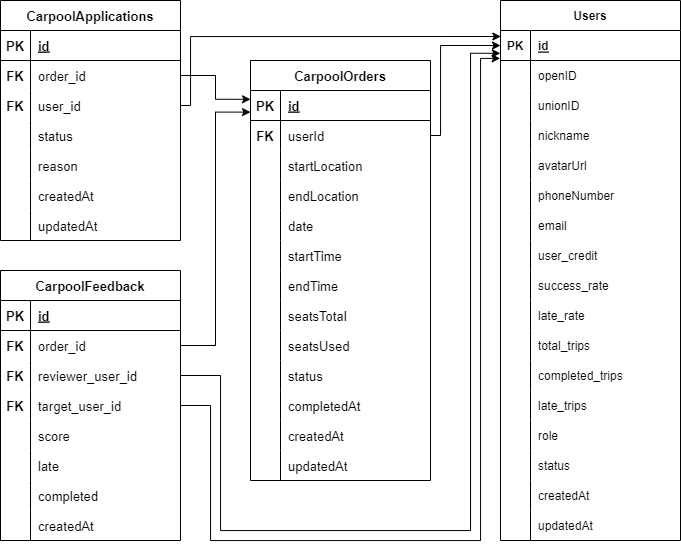
\includegraphics[width=0.94\textwidth]{figures/fig-4-6-mysql-er.png}
  \caption{MySQL数据库核心业务表ER图}
  \label{fig:mysql-er}
\end{figure}

ER图显示了用户表与拼车订单、申请及反馈表的逻辑关系。在实际数据库中，各表独立存储，ER图主要用于说明业务逻辑关联和数据流向。

\begin{table}[!htbp]
  \caption{用户表}
  \label{tab:users-table}
  \centering
  \small
  \begin{tabular}{p{3.0cm}p{2.3cm}p{7.0cm}}
    \toprule
    字段名 & 类型 & 含义 \\
    \midrule
    id & BIGINT & 用户主键，自增 \\
    openID & VARCHAR & 微信OpenID，唯一标识用户 \\
    unionID & VARCHAR & 微信UnionID \\
    nickname & VARCHAR & 用户昵称 \\
    avatarUrl & VARCHAR & 用户头像地址 \\
    phoneNumber & VARCHAR & 手机号 \\
    email & VARCHAR & 邮箱 \\
    user\_credit & DOUBLE & 用户信用评分，默认1.0 \\
    success\_rate & DOUBLE & 拼车完成率，默认1.0 \\
    late\_rate & DOUBLE & 迟到率，默认0 \\
    total\_trips & INT & 参与拼车总次数 \\
    completed\_trips & INT & 成功完成拼车次数 \\
    late\_trips & INT & 迟到次数 \\
    role & VARCHAR & 用户角色，默认USER \\
    status & VARCHAR & 用户状态，默认ACTIVE \\
    createdAt & DATETIME & 创建时间 \\
    updatedAt & DATETIME & 更新时间 \\
    \bottomrule
  \end{tabular}
\end{table}

\begin{table}[!htbp]
  \caption{拼车订单表}
  \label{tab:carpool-order-table}
  \centering
  \small
  \begin{tabular}{p{3.0cm}p{2.3cm}p{7.0cm}}
    \toprule
    字段名 & 类型 & 含义 \\
    \midrule
    id & BIGINT & 拼车订单主键，自增 \\
    userId & BIGINT & 发布订单的用户ID \\
    startLocation & VARCHAR & 出发地点 \\
    endLocation & VARCHAR & 目的地点 \\
    date & DATE & 拼车日期 \\
    startTime & TIME & 期望开始时间 \\
    endTime & TIME & 期望结束时间 \\
    seatsTotal & INT & 总座位数 \\
    seatsUsed & INT & 已占用座位数 \\
    status & VARCHAR & 订单状态，OPEN、COMPLETED、DELETED \\
    completedAt & DATETIME & 订单完成时间 \\
    createdAt & DATETIME & 创建时间 \\
    updatedAt & DATETIME & 更新时间 \\
    \bottomrule
  \end{tabular}
\end{table}

\begin{table}[!htbp]
  \caption{拼车申请表}
  \label{tab:carpool-application-table}
  \centering
  \small
  \begin{tabular}{p{3.0cm}p{2.3cm}p{7.0cm}}
    \toprule
    字段名 & 类型 & 含义 \\
    \midrule
    id & BIGINT & 主键，自增 \\
    order\_id & BIGINT & 对应拼车订单ID \\
    user\_id & BIGINT & 申请用户ID \\
    status & VARCHAR & 申请状态，WAIT、PASS、REFUSE \\
    reason & VARCHAR & 拒绝原因或说明 \\
    createdAt & DATETIME & 创建时间 \\
    updatedAt & DATETIME & 更新时间 \\
    \bottomrule
  \end{tabular}
\end{table}

\begin{table}[!htbp]
  \caption{拼车反馈表}
  \label{tab:carpool-feedback-table}
  \centering
  \small
  \begin{tabular}{p{3.0cm}p{2.3cm}p{7.0cm}}
    \toprule
    字段名 & 类型 & 含义 \\
    \midrule
    id & BIGINT & 主键，自增 \\
    order\_id & BIGINT & 对应拼车订单ID \\
    reviewer\_user\_id & BIGINT & 评价人用户ID \\
    target\_user\_id & BIGINT & 被评价人用户ID \\
    score & DOUBLE & 评分，0\textasciitilde1 \\
    late & BOOLEAN & 是否迟到 \\
    completed & BOOLEAN & 是否完成拼车 \\
    createdAt & DATETIME & 评价创建时间 \\
    \bottomrule
  \end{tabular}
\end{table}

通过上述设计，系统在保证核心拼车业务数据强一致性和事务完整性的同时，实现了微服务之间的独立性和可扩展性。MySQL数据库通过主键索引和联合唯一约束支持高效查询与数据约束，并通过应用层控制实现逻辑外键和事务一致性。

\subsection{MongoDB数据库设计}

本系统使用MongoDB存储内容型和消息型数据，包括论坛帖子与评论、聊天会话与消息、文件记录以及公共交通时刻表。MongoDB的文档模型灵活，适合存储嵌套对象、数组及可变字段，使数据模型更贴合实际业务需求。

\begin{table}[!htbp]
  \caption{帖子集合}
  \label{tab:posts-collection}
  \centering
  \small
  \begin{tabular}{p{3.0cm}p{2.3cm}p{7.0cm}}
    \toprule
    字段名 & 类型 & 含义 \\
    \midrule
    \_id & ObjectId & 文档主键 \\
    userId & String & 发帖用户ID \\
    title & String & 帖子标题 \\
    content & String & 帖子正文 \\
    attachments & Array & 附件列表，每项包含文件地址、类型和上传时间 \\
    tags & Array & 帖子标签 \\
    likes & Int & 点赞数 \\
    commentsCount & Int & 评论数 \\
    createdAt & Date & 创建时间 \\
    \bottomrule
  \end{tabular}
\end{table}

帖子集合主要用于保存论坛中的主题内容。由于帖子通常同时包含标题、正文、标签以及多张图片附件，而不同帖子在标签数量和附件数量上存在明显差异，因此采用文档结构能够更自然地保存这类半结构化数据。在查询实现上，系统主要根据创建时间、标签和发帖用户进行检索，帖子中的点赞数和评论数则以冗余字段形式直接保存在文档中，从而减少列表页查询时的聚合开销。

\begin{table}[!htbp]
  \caption{评论集合}
  \label{tab:comments-collection}
  \centering
  \small
  \begin{tabular}{p{3.0cm}p{2.3cm}p{7.0cm}}
    \toprule
    字段名 & 类型 & 含义 \\
    \midrule
    \_id & ObjectId & 文档主键 \\
    postId & ObjectId & 所属帖子ID \\
    userId & String & 评论用户ID \\
    parentCommentId & ObjectId & 上级评论ID（楼中楼回复） \\
    content & String & 评论内容 \\
    attachments & Array & 评论附件 \\
    likes & Int & 点赞数 \\
    createdAt & Date & 创建时间 \\
    \bottomrule
  \end{tabular}
\end{table}

评论集合用于保存帖子下的回复信息，并支持楼中楼形式的层级评论。通过在评论文档中直接保存 \texttt{postId} 和 \texttt{parentCommentId}，系统能够在不额外设计复杂关联表的情况下完成评论归属和父子关系表达。该结构适合论坛场景中评论数量增长较快、层级关系灵活的特点，同时便于按照帖子维度和时间顺序进行读取。

\begin{table}[!htbp]
  \caption{聊天会话集合}
  \label{tab:chat-collection}
  \centering
  \small
  \begin{tabular}{p{3.0cm}p{2.3cm}p{7.0cm}}
    \toprule
    字段名 & 类型 & 含义 \\
    \midrule
    \_id & ObjectId & 文档主键 \\
    participants & Map & 成员信息（昵称、头像、加入时间、免打扰状态） \\
    lastUpdated & Date & 最近消息更新时间 \\
    \bottomrule
  \end{tabular}
\end{table}

聊天会话集合用于描述会话参与者及会话级状态信息。系统将参与者信息以键值映射形式存储在 \texttt{participants} 字段中，可以直接记录昵称、头像、加入时间和免打扰状态等内容。相较于关系型数据库需要通过多张中间表维护会话成员关系的方式，MongoDB 的文档结构更适合此类成员信息嵌套、字段扩展频繁的场景。

\begin{table}[!htbp]
  \caption{聊天消息集合}
  \label{tab:message-collection}
  \centering
  \small
  \begin{tabular}{p{3.0cm}p{2.3cm}p{7.0cm}}
    \toprule
    字段名 & 类型 & 含义 \\
    \midrule
    \_id & ObjectId & 文档主键 \\
    chatId & ObjectId & 所属会话ID \\
    senderId & String & 发送者ID \\
    type & String & 消息类型（TEXT、IMAGE、FILE） \\
    content & String & 消息内容或文件地址 \\
    timestamp & Date & 发送时间 \\
    userStatuses & Map & 用户状态（isRead、isDeleted、readAt） \\
    \bottomrule
  \end{tabular}
\end{table}

聊天消息集合用于保存具体的通信内容及不同用户对消息的状态标记。消息类型可能为文本、图片或文件，且同一条消息对不同用户还存在已读、删除等个性化状态，因此使用文档数据库可以将消息主体和状态信息组织在同一文档中，减少额外状态表设计。系统在消息查询时主要按照 \texttt{chatId} 和时间戳进行排序读取，从而支持会话页面按时间顺序展示聊天记录。

总体来看，MongoDB 在本系统中主要承担论坛内容与即时消息数据的存储任务。其文档模型能够较好适应字段结构灵活、嵌套关系明显和读写频率较高的业务特点，同时配合 \texttt{\_id}、时间字段及业务检索字段上的索引设计，可以满足系统在帖子列表、评论读取和聊天消息查询场景下的性能需求。

\section{接口设计}

本系统接口设计遵循RESTful风格，统一采用“/api/\{module\}/\{action\}”的路径规范，通过HTTP方法区分操作类型。接口数据交互统一采用JSON格式，并采用标准化返回结构，以保证系统的可扩展性与前后端协作的一致性。根据系统功能划分，接口设计主要包括用户模块、论坛模块、拼车模块、聊天模块以及交通模块五个部分。

\subsection{用户模块接口设计}

用户模块负责管理系统的用户身份、个人信息以及与拼车服务相关的信用统计信息。在校园综合交通场景中，用户是所有业务流程的核心，用户模块接口不仅保证身份认证的安全性，还为其他模块提供统一的用户信息访问和操作入口。通过接口设计，系统能够实现用户登录状态的管理、个人资料的更新与查询、系统通知的获取以及拼车相关行为数据的统计，从而支撑平台的完整功能。

\begin{table}[!htbp]
  \caption{用户模块接口}
  \label{tab:user-api}
  \centering
  \small
  \begin{tabular}{p{1.6cm}p{4.6cm}p{6.2cm}}
    \toprule
    方法 & 接口路径 & 功能说明 \\
    \midrule
    POST & /api/user/login & 微信授权登录，获取用户身份信息 \\
    GET & /api/user/getProfile & 获取当前用户个人资料 \\
    PUT & /api/user/updateProfile & 更新用户基本信息（头像、昵称等） \\
    GET & /api/user/getNotices & 获取系统通知列表 \\
    PUT & /api/user/updateCarpoolStats & 更新用户拼车信用、成功率、迟到率 \\
    \bottomrule
  \end{tabular}
\end{table}

\subsection{论坛模块接口设计}

论坛模块接口主要支持校园用户之间的信息发布与互动交流。系统提供帖子列表查询与详情查看接口，实现对帖子数据的分页加载与精细化展示，满足用户浏览需求。

\begin{table}[!htbp]
  \caption{论坛模块接口}
  \label{tab:forum-api}
  \centering
  \small
  \begin{tabular}{p{1.6cm}p{4.6cm}p{6.2cm}}
    \toprule
    方法 & 接口路径 & 功能说明 \\
    \midrule
    GET & /api/forum/listPosts & 获取帖子列表（支持分页） \\
    GET & /api/forum/getPostDetail & 获取帖子详细信息 \\
    POST & /api/forum/createPost & 发布帖子（支持图片） \\
    DELETE & /api/forum/deletePost & 删除帖子 \\
    POST & /api/forum/setPostLike & 点赞或取消点赞 \\
    GET & /api/forum/listComments & 获取评论列表 \\
    POST & /api/forum/createComment & 发布评论 \\
    DELETE & /api/forum/deleteComment & 删除评论 \\
    GET & /api/forum/listUserPosts & 获取用户发布的帖子 \\
    \bottomrule
  \end{tabular}
\end{table}

\subsection{拼车模块接口设计}

拼车模块是平台的核心业务模块，支持拼车信息的发布、申请、匹配和行程管理。接口设计围绕完整的拼车生命周期展开，包括发布拼车、匹配推荐、申请管理以及行程完成后的反馈统计。

\begin{table}[!htbp]
  \caption{拼车模块接口}
  \label{tab:carpool-api}
  \centering
  \small
  \begin{tabular}{p{1.6cm}p{4.6cm}p{6.2cm}}
    \toprule
    方法 & 接口路径 & 功能说明 \\
    \midrule
    GET & /api/carpool/listOrders & 查询拼车列表（含模型排序推荐） \\
    GET & /api/carpool/getOrderDetail & 获取拼车详情 \\
    POST & /api/carpool/createOrder & 发布拼车信息 \\
    DELETE & /api/carpool/deleteOrder & 删除拼车 \\
    POST & /api/carpool/createApplication & 提交拼车申请 \\
    GET & /api/carpool/getApplicationStatus & 查询申请状态 \\
    GET & /api/carpool/listOrderApplications & 获取某拼车的申请列表 \\
    POST & /api/carpool/approveApplication & 车主通过申请 \\
    POST & /api/carpool/rejectApplication & 车主拒绝申请 \\
    DELETE & /api/carpool/deleteApplication & 撤销拼车申请 \\
    GET & /api/carpool/listUserOrders & 获取我发布的拼车 \\
    GET & /api/carpool/listJoinedOrders & 获取我参与的拼车 \\
    POST & /api/carpool/completeOrder & 标记拼车行程完成 \\
    GET & /api/carpool/listFeedbackTargets & 获取待评价对象 \\
    POST & /api/carpool/submitFeedback & 提交拼车评价并更新信用 \\
    \bottomrule
  \end{tabular}
\end{table}

\subsection{聊天模块接口设计}

聊天模块接口用于实现用户之间的即时通信功能。接口设计覆盖会话列表、消息获取与发送、已读标记、消息删除等功能，实现数据一致性与高效通信，同时满足社交互动和通知需求。

\begin{table}[!htbp]
  \caption{聊天模块接口}
  \label{tab:chat-api}
  \centering
  \small
  \begin{tabular}{p{1.6cm}p{4.6cm}p{6.2cm}}
    \toprule
    方法 & 接口路径 & 功能说明 \\
    \midrule
    GET & /api/chat/listUserChats & 获取用户会话列表 \\
    POST & /api/chat/createChat & 创建或复用单聊会话 \\
    GET & /api/chat/listMessages & 获取聊天消息列表 \\
    POST & /api/chat/sendMessage & 发送消息 \\
    PUT & /api/chat/markRead & 标记消息为已读 \\
    PUT & /api/chat/deleteMessage & 删除单条消息 \\
    PUT & /api/chat/addParticipant & 添加会话成员 \\
    \bottomrule
  \end{tabular}
\end{table}

\subsection{交通模块接口设计}

交通模块用于提供校园班车及公交信息查询功能，为用户出行提供基础数据支持。

\begin{table}[!htbp]
  \caption{交通模块接口}
  \label{tab:transport-api}
  \centering
  \small
  \begin{tabular}{p{1.6cm}p{4.6cm}p{6.2cm}}
    \toprule
    方法 & 接口路径 & 功能说明 \\
    \midrule
    GET & /api/transport/getNearestBusTime & 获取最近发车时间 \\
    GET & /api/transport/getTimetables & 获取完整公共交通时刻表 \\
    \bottomrule
  \end{tabular}
\end{table}

\section{本章小结}

本章完成了系统总体架构、模块划分、数据库结构和接口组织方式的设计说明。通过前后端分离、微服务拆分以及混合存储方案的配合，系统在功能协同、数据组织和后续扩展方面形成了较清晰的实现基础。
